
\section{Study1: Entity-Centric Foraging across Browser Tabs}

\begin{figure}
    \centering
    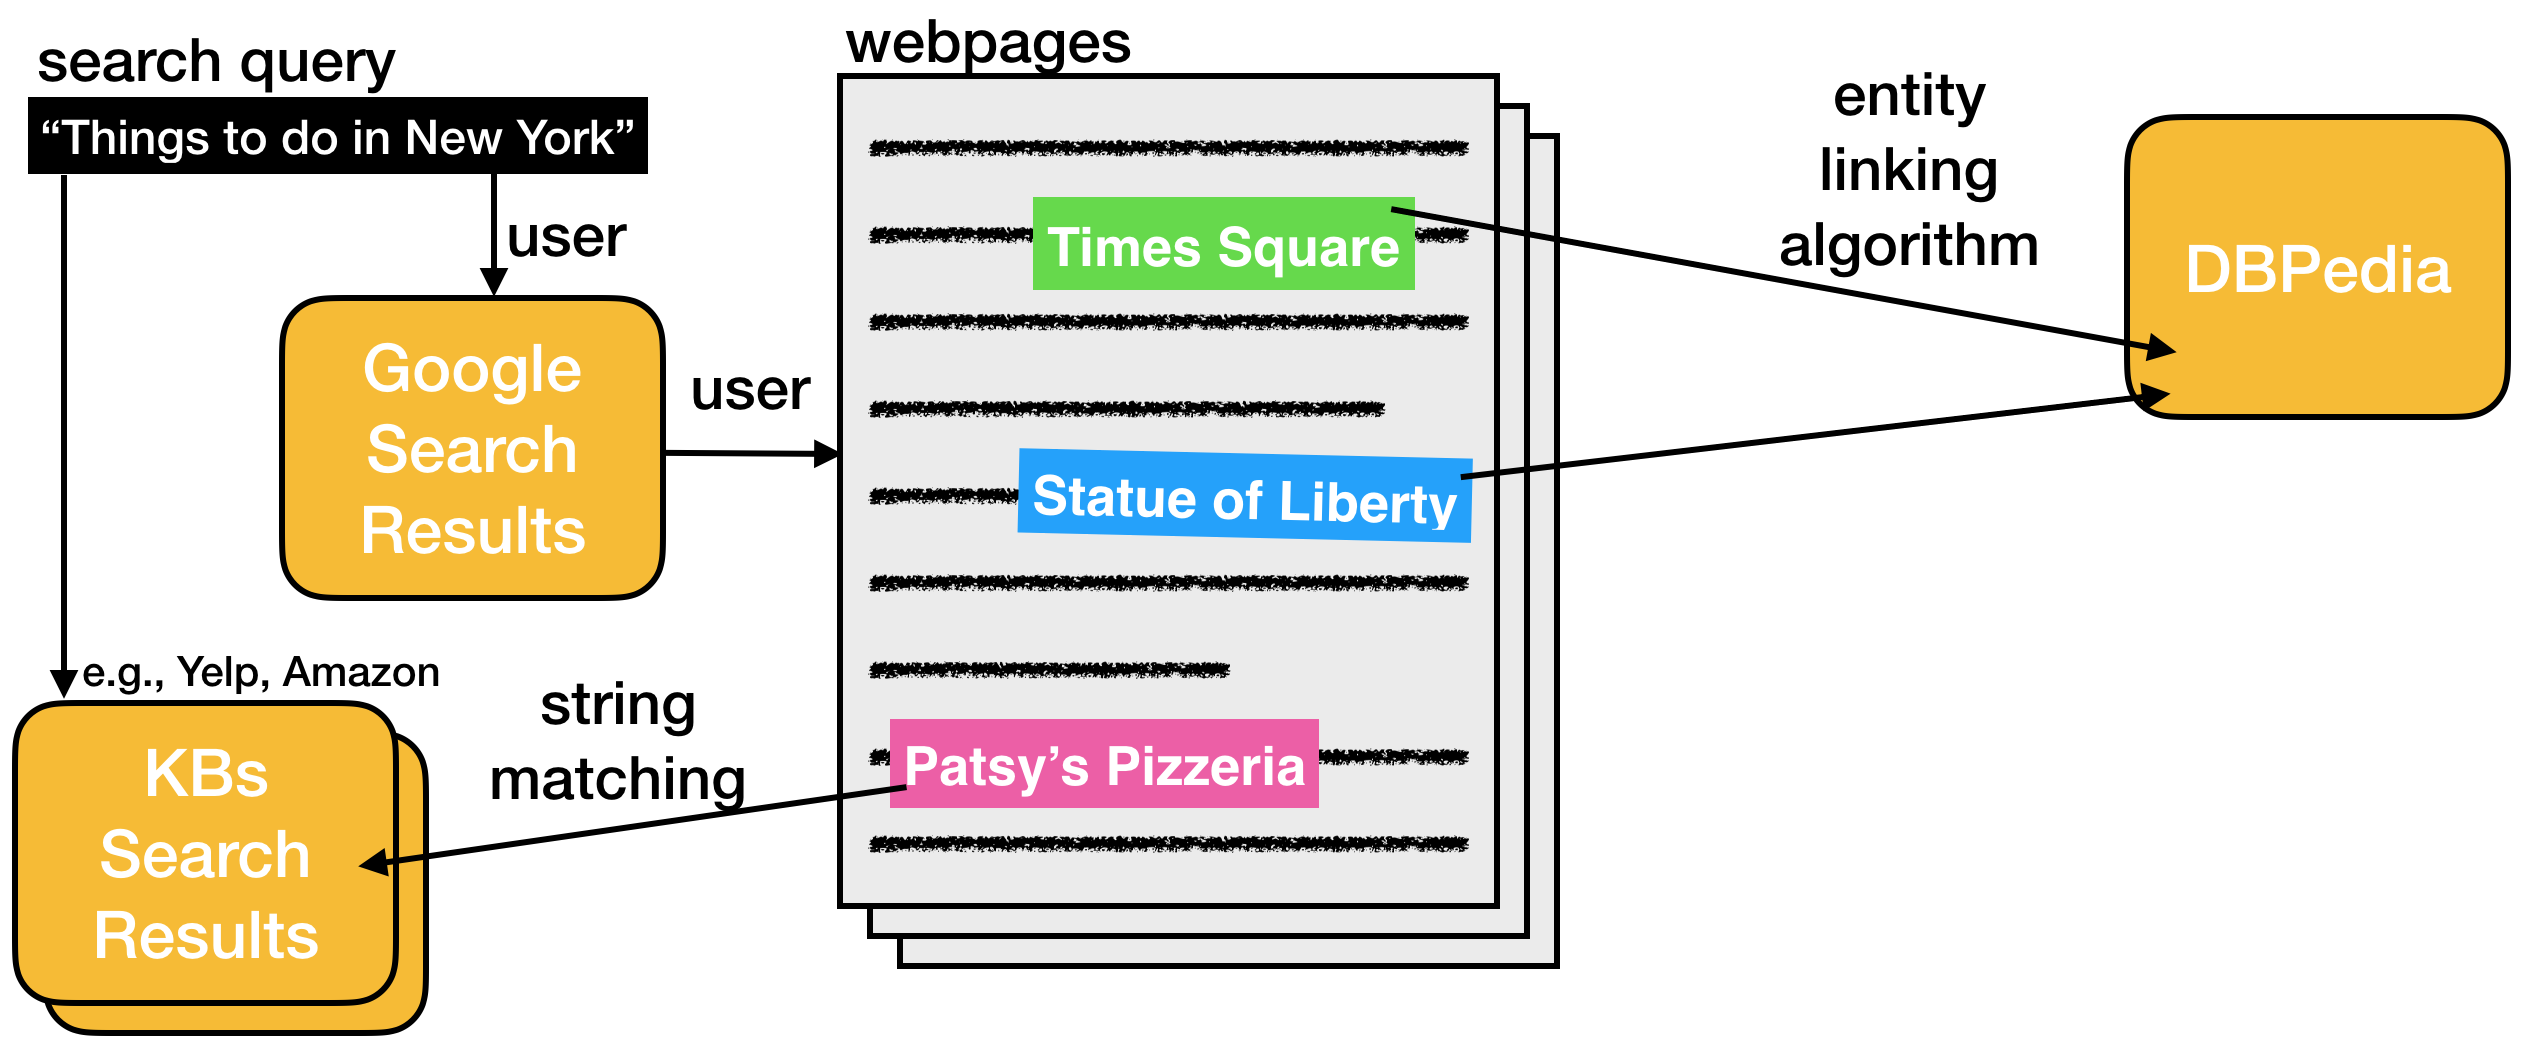
\includegraphics[width=0.7\textwidth]{images/linking.png}
    \caption{The proposed work will use entity linking algorithms to identify Wikipedia entities mentioned in different webpages, combined with querying multiple other knowledge bases using users' original search query to improve recall.}
    \label{fig:linking}
\end{figure}


The goal of Study 1 is to explore an alternative design space where the browser is able to identify and connect the same options and evidence mentioned across different webpages and use this understanding to provide better support for foraging and structuring information when users conduct exploratory search tasks. To enable this, I will develop a browser extension that incorporates existing knowledge bases and entity linking algorithms (such as \cite{spotlight,dbpedia}) and equips the browser the ability to recognize entity options from webpages. The tradeoff here is that using existing knowledge bases instead of crowdsourcing for identifying options (i.e., \cref{chap:alloy}) will allow me to develop and release a system to test this idea at scale at the cost of limited scenarios, but still support for a variety of different tasks covered by entities from Wikipedia \cite{dbpedia}, the Yelp API, or the Google Knowledge Graph API. Figure \ref{fig:linking} shows the proposed framework for identifying common options from multiple webpages in an exploratory search. For open domain knowledge bases (such as Wikipedia), I will use existing entity linking algorithms to analyze text and identify entity mentions. This will allow the system to resolve different surface forms of the same entity. To support knowledge bases where entity linking algorithms were not available but still provide search APIs (such as Yelp or Google Knowledge Graph), I propose to query each for a list of relevant entities using the original query terms the user submitted to a search engine, and use string matching to identify entity mentions in webpages.


By enabling the browser to connect webpages through option mentions, we can help users gather and synthesize evidence about entities across multiple webpages and gradually build up a workspace that persists across browser tabs throughout the task. This approach has the potential to not only reduce the costs of keeping track of options and gathering evidence, but also enables new end-user interface designs, such as proactively showing a user how many sources mention an entity and the contexts in which it was mentioned, or propagating an users' notes and annotations across all pages an entity was cited.
The key insight we build on is that while users aim to collect evidence for entities across multiple sources, current browsers treat each of the instances of those entities as independent. If we instead understood that the same entity was being mentioned on multiple different pages, we could better support users in understanding the contexts that entity was mentioned in and allow them to cross-reference between different sources and their own notes efficiently.


%\section{Preliminary: The Cost Structures of Tab Usage}
%\label{chap:tabs}
%
To better understand ways to support this process, this chapter describe a preliminary study on the common issues and limitations of tabbed browsing during complex productivity tasks. 
Tabs have become an integral part of how people browse and navigate the web since they were introduced in the early 2000s, and they are now a ubiquitous feature in all major web browsers. However, since their introduction, the internet has gone through dramatic changes, with an increasing proportion of users' communication, productivity, and entertainment tasks moving from the desktop to ``\emph{the cloud}'' \cite{Dubroy:2010:STB:1753326.1753426}. Further, online information seeking has evolved from navigating web directories to finding websites (e.g. DMOZ \cite{dmoz}) for simple fact finding tasks to searching through dozens or even hundreds of webpages to support complex sensemaking tasks \cite{pirolli1999information,marchionini2006exploratory}. These changes reflect an increasing amount of dependence on the functionality and interfaces of modern web browsers in meeting these needs.

However, despite this expansion of functionality, there have been few changes to the way tab interfaces are designed today versus when they were introduced. Tabs are now simultaneously used to check email inboxes, view videos, control music players, stash articles to read later, chat with friends, plan trips, research products, write articles, and work on projects. Yet even with this diverse and multifaceted set of functions, tabs still remain instantiated as simple temporally-ordered lists with few contextual cues. Indeed, the fixation on tabs as a metaphor is so strong that the most popular changes to using tabs involve relatively small design adjustments such as making them a vertical instead of horizontal list \cite{vtabs} or creating tabs that contain more tabs \cite{treetabs}. 
There is increasing evidence that using tabs for this wide array of functions leads to breakdowns, overload, and missed opportunities \cite{web1, web2, web3, web4, web5}.
To better understand and expand the potential design space for web browsing interfaces, we conducted an empirical study of the challenges people face when using tabs. Instead of examining the specific functions of tabs as they are currently used (e.g., as in Dubroy, 2010 \cite{Dubroy:2010:STB:1753326.1753426}), we focus on developing a model of the way that tabs break down from their daily use. We performed both an online survey and in-person interviews to investigate and build this model.

We found that participants' behavior was governed by a variety of positive and negative drivers. Overall, these drivers could be classified as two opposing forces: pressures to close tabs, and pressures to keep tabs open.  We found strong evidence that participants had numerous reasons to close their tabs, ranging from limited attention to limited browser resources to self presentation.  At the same time, we found a diverse set of reasons why it was not so simple to close open tabs. These included previously reported drivers such as reminding users of unfinished tasks \cite{Dubroy:2010:STB:1753326.1753426}, but also new factors relating to cost structure of tabbed browsing, such as the cost of reaccessing pages, the sunk costs of finding and organizing information, the benefits of supporting an (unrealistic) aspirational self, and the uncertainty of the expected value of information in the future, especially for complex tasks. These pressures to close vs. keep open tabs interact to create feelings of stress, being overwhelmed, and even shamefulness in our participants. Our findings have implications for the design of new forms of web browsing that can better support the underlying drivers behind the use of tabs.

\begin{table*}
\centering
\footnotesize
  \def\arraystretch{1.1}
  
  \begin{tabular}{l p{11.6cm}}
  
  \hline
  \multicolumn{2}{c}{Different Pressures for Closing Tabs versus Keeping Tabs Opened} \\
  \hline
  
    \textbf{C1}.Limited Attention &
    Keeping too many tabs can be overwhelming and makes it difficult to focus \\
    
    \textbf{C2}.Screen Real-estate &
    Having too many tabs makes it hard to navigate and have situational awareness \\
    
    \textbf{C3}.Computing power &
    Drains processors and memory, causing browser and other applications to slow \\
    
    \textbf{C4}.To be Organized &
    Social and self pressure to avoid looking disorganized \\
    
    \hline
    
    \textbf{O1}.Remind and Resume &
    Keeping tabs around as a reminder to work on them or keep track of progress \\

    \textbf{O2}.Revisit References &
    Keeping frequently used tabs for quick access; has a diminishing return \\
    
    \textbf{O3}.Costly Re-finding &
    Avoid closing tabs in fear of not being able to re-find valuable information \\
    
    \textbf{O4}.Aspiration/Sunk Cost  &
    The hopes to process more information than capable; while aware of the situation \\
    
    \textbf{O5}.Mental Model &
    Tabs and windows represent external memory and mental models for complex tasks \\
    
    \textbf{O6}.Uncertain Relevance &
    Difficulties in judging the current and potential relevance of tabs in the future \\
    
    \hline

  \end{tabular}

  \caption[An overview of our findings in the tab usage study.]{An overview of our findings: Two sets of opposing pressures that drive tabbed browsing behavior.}
  \label{tab:overview}
\end{table*}



\subsection{Online Survey}

An online survey was conducted with 64 participants recruited from the Amazon Mechanical Turk task market (age: M=33.7, SD=10.6, min=19, max=67; 57\% male; 77\% from the US). The survey consists of a demographic questionnaire, a 7 question Maximizer-Satisficer Questionnaire \cite{nenkov2008short}, and 24 questions we designed about users habits and opinions of using tabs. Each of the 31 questions were rated by the participants using a 7-point Likert scale with options ranging from Strongly Disagree (0) to Strongly Agree (6).  The personality trait quiz was originally developed by Schwartz et. al 2002 for measuring how much a person tend to maximize (or optimize) in sensemaking and decision making scenarios \cite{schwartz2002maximizing}. In our survey, we used the short form version of the survey developed by Nenkov et. al in 2011 with 7 questions \cite{nenkov2008short}, which had been found useful in past work for identifying users with different types of online information seeking tendencies \cite{kittur2013costs}. For each participant, we averaged their responses of the 7 personality trait questions to form a scale of 0 to 6, where a higher number indicates someone identifies as more of a maximizer. Participants agreed strongly on 13 of the tab questions, with 95\% confidence interval above the neutral option (3.0 neither agree nor disagree). In addition, we found responses of multiple tab questions to be highly correlated with participants' personality traits. We will show these in the appropriate sections.

\subsection{In-Person Interviews}

Ten participants were recruited from either a university or a research facility located in two states in the US for in-person interviews (age: M=23.0, SD=4.7, min=19, max=32, 40\% male). Most participants were either graduate or undergraduate students conducting research during the summer. Pre-screening was used to recruit participants who self-reported often reaching 12 or more tabs open in their browsers and use a laptop as their main computer. 
Semi-structured interviews were conducted closely following a detailed interview scripts. Participants were asked to walk through each tab they had opened on their laptops with the interviewer, and explain the tasks, goals, or purposes of why each tab was opened in the first place. We then further probe our participants to discuss with us why each tab was still opened, using questions including ``\emph{Was this tab intentionally kept around for later usage?}'' If answered ``\emph{yes}'', we followed up with ``\emph{Did you came back to it recently, why or why not?}'' And if answered ``\emph{no}'', we followed up with ``\emph{Why was this tab kept around if you did not plan to use it again?}'', and ``\emph{Do you struggle to close your tabs?}''  We also asked about how and how effective are they managing their tabs with questions include ``\emph{How frequently do you evaluate your tabs to see if you can close them? How difficult is it?}'', and ``\emph{Does the number of tabs you have opened affect how you feel?}'' The interviews were recorded and transcribed. The authors then extracted and analyzed interested quotes using a grounded theory approach with four rounds of discussions and iterative coding \cite{strauss1998basics}.


\subsection{Pressures to Close vs. Keep Open Tabs}

Overall we found that people had mixed feelings about their tabs. Participants were positive about browser tabs when compared to only using application windows. These findings were consistent with a study on Firefox users in 2010 \cite{Dubroy:2010:STB:1753326.1753426}. 
%Specifically, our participants expressed how tabbed browsing allowed them to load and access many webpages in parallel, while not generating a lot of application windows that can potentially clutter their desktop environment.
However, many participants experienced major issues when trying to manage tabs efficiently. Specifically, when too many tabs were opened, participants expressed feeling negative emotions and pressure. At the same time participants also expressed feeling an attachment to the information saved in tabs and an investment in the organization they built up. Table~\ref{tab:overview} shows an overview of our findings, and below we discuss these two opposing forces that govern users' tab behavior based on evidence from our interviews and survey.


When participants had too many tabs opened, they expressed a number of negative feelings and reasons behind them. Investigating this we found three common themes: tabs incurring pressure on attention; tabs taking up browser resources; and people feeling a desire to appear organized to themselves or others. %On the surface, the linear structure of browser tabs seems to allow users to open, retain, and manage an infinite number of webpages. We argue that there are in fact different implicit costs associated with creating new tabs to load more webpages, and that browser tabs should be considered a \emph{limited resource}. Below we discuss these in more depth.

\subsubsection{C1.Pressure on Attention}

A fundamental problem is people's \emph{limited attention}. In situations where users are presented with too many options, and faced with too many decisions to make, it becomes harder to focus on what is important \cite{schwartz2004paradox,wilson2008improving}. Similarly, having opened too many tabs can potentially cause users to lose track of all the information sources they have on hand, and lose focus on which tabs they should concentrate on. Many participants in our interview study expressed how they were sometimes overwhelmed by the large number of tabs they have opened, and how it made them unable to focus on important tasks.

\begin{quote} 
``\emph{I think probably, overwhelming is a good word. It's not like it's helping, it's not like I can suddenly find things better when I have that many tabs open because that's definitely not the case, so yeah I think the more tabs I have open then it's more an indication that I'm in some, some uh shit, like I'm like in the middle of a mix and like just don't have time for like basic human cleaning functions or something.}'' - Participant J3

\end{quote}

Conversely, participants also pointed to how closing and reducing the number of tabs can relieve pressure and stress caused by their browser tabs. 

\begin{quote}
``\emph{[on closing browser tabs and windows] Usually it's a relief, even if I'm missing things that I think would have been important. I can't usually remember specifically what they would have been.... Yes. When I close a window also. I feel like that's great.}'' - Participant J2
\end{quote}


\subsubsection{C2\&C3.Pressure on Computing and Screen Real-estate}

Besides limited attention, many participants also mentioned \emph{screen real-estate as another limited resource}. They expressed how having too many tabs leads to difficulties in navigating and finding previously opened tabs. More specifically, creating each additional tab reduces the width of existing tabs causing a smaller portion of the webpage titles to be rendered by the browser. Further, they pointed to a breaking point for tabbed browsing: When browser tabs became so narrow that the favicons were no longer rendered, tabbed browsing became unusable. 

%\begin{quote}
%``\emph{so it's kind of a mix between bookmarks and traditional tabs. and I think breaking down that barrier is more useful.  obviously if you have this many tabs, if it were horizontal like you just couldn't read any of it.  here however many tabs I have I can see what's up.}'' - Participant J4
%\end{quote}

\begin{quote}
``\emph{Sometimes, if it gets to so many that I can't even see the icons anymore, then I start closing them.}'' - Participant H3
\end{quote}

%\begin{quote}
%``\emph{So, usually I would group...I don't like it when it gets so tiny you can no longer see the little favicon. So usually I would group thematically.}'' - Participant J3
%\end{quote}

\begin{quote}
``\emph{When I can't see the little icon. Then that's too many... I can definitely find what I want with like 3 clicks at most, generally 1 click. It's once I can't see the little icons...}'' - Participant H4
\end{quote}

\begin{quote}
``\emph{As for like a mental burden...It's crazy. This doesn't happen very often, but if I have enough that the titles or icons don't show, I'll be like, ``Wow, how did I get this bad?'' And get really bothered by it}'' -  Participant H2
\end{quote}

Echoing participants in the interview study, 28\% of the participants  in the survey study also agreed that they \emph{often struggle with finding the tab they needed in their browser} (M=2.17, 95\% CI[1.74, 2.60]). Even though this issue was not reported by the majority of our participants, the responses were highly correlated with the maximization personality trait (t=3.38, df=62, p=0.001 based on Pearson's product-moment correlation), indicating that this might be an issue for a particular subset of the population or when conducting tasks that users care a lot about.

Participants who sometimes keep a large number of tabs around mentioned having too many tabs drains the \emph{limited processing power and memory space} from their computers, causing their browsers to became too slow. Supporting evidence were found in both the interview study and the survey study. 25\% of the participants in the survey study reported that they have experiences with \emph{browser or computer crashing in the past due to having too many browser tabs opened} (M=1.89, 95\% CI[1.40, 2.38]). Similarly, even though the average agreement were relatively low, the responses were highly correlated with the maximization personality trait (t=2.99, df=62, p=0.004 based on Pearson's product-moment correlation). One participant in the interview study, J4, even described how it inhibited him or her from using other desktop applications normally. 

\begin{quote}
``\emph{I'll try to go into different browsers to see if there are tabs that I just don't need. so yeah usually the only time that I do that is if Chrome is starting to get really slow.}'' - Participant J2

\end{quote}
\begin{quote}
``\emph{But right now, I can't, my battery drains so fast because I have all these tabs open, that it actually inhibits a lot of things I'm doing.}'' - Participant J3
\end{quote}
%\begin{quote}
%``\emph{there is a noticeable performance drop the more tabs I have, and because I use LastPass for password management, I think when I hit some number over 100 it starts bugging out a little bit}'' - Participant J4
%\end{quote}

Browser extensions such as \cite{suspend1} and \cite{suspend2} allow users to manually unload and reload webpages while keeping their tabs open to save memory usage has a combined of more than 1.2 million users (as of September, 2017). While they can ameliorate the pressure of using too much processing power, they also introduce another layer of caching that users have to manually manage, and does not help with pressures caused by depleting screen real-estate or user attention.

\subsubsection{C4.Pressure to be Organized}

When conducting tabbed browsing, depleting the different limited resources mentioned above created major issues for our participants. Indeed, many participants described how browser tabs can become a source of stress and frustration due to these limitations, especially when they try to navigate and manage many tabs in parallel.

\begin{quote}
``\emph{... but if it seems like I have a lot of tabs open, I try and go through and see which ones I can close. But sometimes, that's very frustrating because sometimes it's like, well, I can't exactly close any of these right now, but there are so many of them}'' - Participant H1
\end{quote}

More interestingly, some even noted feelings of \emph{shamefulness} for having a large number of tabs opened, and their unwillingness to reveal their tabs to others.

\begin{quote}
``\emph{Because it's...shameful in a way. It makes, like I feel like I would have been giving, like a bad impression to these people that I, that had to look at my screen.}'' - Participant J3

\end{quote}
\begin{quote}
``\emph{i'm going to do a presentation and I care about what people are going to think about me when I plug my computer in, then that's when I might clean it up}'' - Participant J2
\end{quote}

These results suggest that users are in fact motivated to maintain a clean and organized workspace, but were often failing to do so while conducting tabbed browsing. 56\% of the participants from the survey study agreed that \emph{it would be helpful if the browser somehow knew I was done using a tab} (M=3.4*, 95\% CI[3.04, 3.93], highly correlated with the maximization personality trait t=2.08, df=62, p=0.042 based on Pearson's product-moment correlation). Participants also associated the pressure to be organized with social pressure and impression management, and how they would attempt to reduce the number of tabs they have opened before showing others their screens. This could potentially demotivate users to collaborate in-person with their co-workers in a office setting or even remotely using screen-casting tools \cite{birnholtz2012distance}.


%More generally, 50\% of the time half of our participants had less than 6 tabs opened, while the other half had more than or equal to 6 tabs opened, and 25\% of the participants had more than 17 tabs opened 10\% of the time  (Figure~\ref{fig:numOfTabs}).




Given the above pressures caused by having too many tabs, and the seemingly low cost of closing tabs to relieve such pressure, why do participants still frequently find themselves in situations where they ``\emph{hoard}'' many tabs?  Close examination of the interview transcripts revealed 6 major causes for why people open and keep a large number of tabs, many of which were dependent on the usefulness and relevance of a tab over time, leading to issues such as keeping around obsolete tabs that could have been safely closed.



\subsubsection{O1.Reminders and Unfinished Tasks}

Most commonly, participants in the survey study reported that some of their tabs were intentionally kept around for reminding or to keep track of progress:

\begin{itemize}

    \item \emph{as reminders to go back to something}: 86\% agreed, M=4.89*, 95\% CI[4.59, 5.19]
    \item \emph{to continue collect information from}: 91\% agreed, M=4.73*, 95\% CI[4.47, 4.99]
    \item \emph{as reminders to explore further}: 89\% agreed, M=4.70*, 95\% CI[4.44, 4.97]
    \item \emph{to resume where I left off}: 80\% agreed, M=4.41*, 95\% CI[4.08, 4.73]
    \item \emph{tabs correspond to unfinished tasks}: 77\% agreed, M=4.11*, 95\% CI[ 3.77, 4.45] 
    
\end{itemize}

These results based on general tab usage are consistent with previous work that focused on browser tab usage during search sessions \cite{huang2012no}.
Similar responses were also collected from the interviews:

\begin{quote}

``\emph{And sometimes, when you're in a rush, you don't really have time to focus on which tabs you really need, so you'll put it off for later.}'' - Participant H2
\end{quote}

\begin{quote}
``\emph{Yeah it sort serves it not in a ""Oh shit"" way but in more of a, sitting there nagging me like a mother sort of way. And I would say it's effective in doing that.}'' - Participant J3
\end{quote}

Since reminder tabs can be inactive for extended periods, one solution could be to save them as bookmarks so that tab resources can be released. However, participants expressed how bookmarks do not exhibit the same reminding functionality, citing the high cost of creating and accessing bookmarks and that once created they are ``out of sight out of mind''.

\begin{quote}
``\emph{Yeah, I would say bookmarks for me feel like deep archive or something so in Firefox when you bookmark something but you don't assign it to like you don't put it into a folder you just kind of puts it all in a pile}'' - Participant J5
\end{quote}

\begin{quote}
``\emph{I would have to bookmark it and then put it into a category. Would have to save this bookmark and decide which category it would go into. If I bookmark everything, just a default bookmark, it would just get added to a long list of long-forgotten sites that I bookmarked randomly. Because I have bookmarked... I want to bookmark it and put it into a category but then that requires figuring out what category to put it in, which as you know, requires a lot of cognitive load.}'' - Participant J1
\end{quote}

While the task of categorizing and filing personal information requires high cognitive load \cite{lansdale1988psychology},
the structure it creates often bring benefits such as ease of access and a better understanding of the information landscape \cite{strauss1998basics}. However, in this case, forcing users to create structure over their tabs does not seem to exhibit these benefits while still required the high cost of categorization. Additionally, this structure causes tabs to lose their ability to ``nag'' the users from time to time.

\subsubsection{O2.Revisiting Frequently Accessed Pages}

People also keep tabs around to reduce the cost of repeated navigating to frequently revisited webpages. From the survey study, 78\% of our participants agreed that they \emph{keep frequently used tabs opened} (M=4.67*, 95\% CI[4.33, 5.01]), and similar responses were also collected from the interview study:

%\begin{quote}
%``\emph{If i'm going to go back to it so frequently, why would I ever close out of the tab? Why would I ever want to have to reload the tab?}'' - Participant H4
%\end{quote}

\begin{quote}
``\emph{ I do usually try to have one window more of my core stuff, so my window right now has my email, calendar, and capstone stuff that I can reference really quickly. }'' - Participant J2
\end{quote}

However, immediately afterwards J2 noted that the benefit of keeping frequently accessed tabs around has a diminishing return: as the total number of tabs increases, users ability to efficiently access specific tabs decreases. This tension leaves users the heavy burden of carefully balancing between the number of frequently used tabs to keep around, and how efficiently those tabs can actually be accessed. J2 summarized this cost structure balance with an apt analogy to putting clothes away:

\begin{quote}
``\emph{
....think for me it feels like other things that I do that don't make a lot of sense but feel like the right things to do, so like I've often have in my room like a chair that I'll just drape clothes back over the chair instead of putting it away. Cuz if it's a sweater that I wear a few times a week, well it'll be easier if I just get that sweater that's draped over this chair than if I put it in my closet, but then that becomes like 30 things draped over the chair, and I actually can't find anything draped over the chair, and I know it doesn't make sense but I still do it. Like in the moment it seems like the right thing to do, the easier thing to do.}'' - Participant J2
\end{quote}



\subsubsection{O3.Avoiding Costly Re-finding}

Besides keeping tabs open to reduce revisitation costs, participants also noted how \emph{closing tabs} can potentially incur the high costs of re-finding and reopening them, and how they kept tabs around in order to avoid such scenarios.


\begin{quote}
``\emph{like if I close a window but I want those tabs back it's probably in history somewhere I just... it used to be really shaky so I never did it.}'' - Participant H5
\end{quote}



	
%\begin{quote}
%``\emph{I didn't want to close it because I want to make sure that it worked before I did, and I didn't reference it again once I saw that it worked.}'' - Participant J2
%\end{quote}


The cost of reopening tabs was often mentioned with online collaboration. Participants noted that when tabs were open from links shared by others, the costs of reopening are often higher, so they were less likely to close them.

\begin{quote}
``\emph{Because I'm not confident I know how I would get back to it. Especially if it was a link that I followed from Slack\footnote{Slack. An instant messaging application. http://www.slack.com} that someone else created in our drive.... in some cases, the files that I've created, I know where they are and so I know where to find them. But in the case of other people's files, I don't know where they are so I am more likely to keep their tabs opens. I am more likely to keep tabs open for files that other people create because I don't know where they filed it.}'' - Participant J1
\end{quote}

%\begin{quote}
%``\emph{sometimes I think they're opening through an email link or a slack link, had it open somewhere else. in the case of my calendar it was probably I was trying to access my calendar quickly and I didn't see that I had it open.}'' - Participant J2
%\end{quote}

%\subsection{Feeling of being invested}

Conversely, many participants expressed their fear of closing the wrong tabs, either by mistake or by misjudging their relevance, and pointed to cases where they had to pay the price of re-find and reopen valuable tabs. One participant even stated that he or she would go through history to find valuable tabs that were closed, while others were willing lose information they considered valuable just to avoid having too many tabs. 

\begin{quote}
``\emph{But in all likelihood there's been a few tabs where I've saved and I've never come back to. Or it gets closed out accidentally. Which is a very scary... or a fear of mine where a tab will get closed out and I won't know what I'm missing.... It's the fear of missing something important, or something that will lead to enlightenment, or to more knowledge, or something that will help you get a job. Things like that. Just the fear of missing out.}'' - Participant J1
\end{quote}

\begin{quote}
``\emph{...I would actually go through my browsing history and go "I had this tab open, I had this tab open, I had this tab open" and then I would reopen a lot of those tabs.}'' - Participant J4
\end{quote}

As a result, one participant also noted how using external note taking application to record URLs before closing tabs can lower the potential cost of re-opening them.

\begin{quote}
``\emph{Right and if we were doing something like cancer research or something, I would paste a lot of links in so then I don't necessarily keep those tabs open. If I get it recorded then I can close things.}'' - Participant J5 
\end{quote}

\subsubsection{O4.``Irrational'' Pressures: Sunk Costs \& the Aspirational Self}

Participants also cited reasons for keeping tabs around that may not fit in a rational economic analysis view of the cost structures of tab usage. Two common patterns were the sunk cost of creating and managing tabs, and the disparity between a participant's actual and aspirational self.

\emph{Sunk Cost}. When participants spent efforts to open, manage and organize their tabs, they feel invested  and felt that those tabs had inherent value to them beyond just the costs and benefits of keeping them around for quick access or to avoid re-finding them. This reluctance to close tabs may be a form of loss aversion \cite{tversky1991loss}, in which simply the ``ownership'' of a tab may give it value:

\begin{quote}
``\emph{But it made me think about how it's weird that even when I'm not using those tabs, I don't want to close them. Maybe it's because it took effort to open those tabs and organize them in that way}'' - Participant H2
\end{quote}

Another form of ``irrational'' behavior reminiscent of loss aversion we found was the mismatch between a participant's goals for their aspirational self and what would be realistic for their actual self. For many tasks there are virtually an unlimited amount of relevant information given the scale of the modern Web. Users with a maximization tendencies may spent huge amounts of time collecting information to avoid the chance of missing valuable insights. Furthermore, users often encountered a variety of interesting articles or websites in their social media or news feeds that they would like to read someday. Indeed, participants reported that sometimes the amount of information they hoped to process exceeds their capability and resources. 


\begin{quote}
``\emph{...it's not really worth it. But at the same time, I don't want to be like ``Oh, okay, that's it. I'll never remember.'' So I just leave it there. And then I might not come back to it}'' - Participant H4
\end{quote}

\begin{quote}
``\emph{it kind of becomes this kind of mess that you see here, just a big list of tabs that I was supposed to get back to but never did.}'' - Participant J4
\end{quote}


%\begin{quote}
%``\emph{Yeah it sort serves it not in a ""Oh shit"" way but in more of a, sitting there nagging me like a mother sort of way.}'' - Participant J3
%\end{quote}


\begin{quote}
``\emph{I'm sure somewhere in that 100 there were some things that were really important for me to keep in my mind. But now they're gone. So "oh well" I guess.}'' - Participant J3
\end{quote}

Interestingly, when asked if they would ever get to processing a certain resource some participants admitted that realistically they would never actually get to them.

\begin{quote}
``\emph{to be honest,  it's more like I will collect a bunch of links and then never really ever go back to them. And when I figured this out I sort of stopped caring about bookmarks.  sometimes I will throw things into this other bookmark that's more unorganized,  but I don't think I ever look back on these.}'' - Participant J4
\end{quote}


%\begin{quote}
%``\emph{But in all likelihood there's been a few tabs where I've saved and I've never come back to.  Or it gets closed out accidentally. Which is a very scary... or a fear of mine where a tab will get closed out and I won't know what I'm missing.}'' - Participant J1
%\end{quote}


\subsubsection{O5.External Mental Model}

%Even though web browsers typically only provide a simple linear structure for organizing tabs, our participants were still using tabs to manage multiple complex tasks in parallel. Indeed, 

Participants expressed how browser tabs act as a manifestation of their mental models, using them as an external -- yet transient -- memory store in a similar fashion as an active working memory \cite{baddeley1974working}.

\begin{quote}
``\emph{It's like a manifestation of everything that's on my mind right now I think. Or the things that I think need to be on my mind right now, I think that's the way I think about it. Like, so right now, in my browser window, I have like, a web project that I'm working on. I don't have time to work on it right now, but I know I need to work on it, so it's sitting there kind of reminding me that I need to work on it.}'' - Participant J3
\end{quote}

Our participants typically conducted a wide range of different tasks in parallel, sometimes engaging in multiple productivity and leisure tasks at the same time. 
%\begin{quote}
%``\emph{I just opened it in Firefox and I kind of had Hulu and Netflix open there and it felt like it was good to keep it separate from my more serious work related tasks. Like I wouldn't get distracted if I'm in like a this one... I wouldn't see the little Netflix icon and get tempted.}'' - Participant J2
%\end{quote}
The simple linear structure of tabs were often insufficient for organizing multiple complex tasks at the same time, and participants had to resort to various strategies and tools to create more sophisticated structures to better represent their mental models. Participants in our interview reported strategies from using multiple windows to create two-level hierarchies of tabs (as in  \cite{Dubroy:2010:STB:1753326.1753426}) to using virtual desktops and even multiple browsers or computers to create more levels of hierarchies or to separate task contexts. 

%\begin{quote}
%``\emph{I would open Word or I have a research file for this podcast so I would probably do that open that up and a different desktop and then decide what I want to research and then I would come over here and go to this thing and then double-click to create a new group and now we are in a new group so search for something and food and wine is a good resource like wine mag and then I might go to Wikipedia manually or whatever I do my research and I be flipping back and forth to my file here and then when I'm sort of done probably eventually after I recorded I would probably leave this stuff open until I'm done done.}'' - Participant J5
%\end{quote}


\begin{quote}
``\emph{...a lot of the times I have are for entertainment and reference and something that I need to get back to. whereas my Mac is for work. I'll just call it my home computer and my work computer. if I had my tabs on my home computer on my work computer I will probably get more distracted. this is more for fun and my work computer is for work.}'' - Participant J4
\end{quote}

\begin{quote}
``\emph{I would usually try to keep either different windows or often I would have different browsers like Chrome at work and Firefox at home so that I wouldn't mix those things up.}'' - Participant J2
\end{quote}

%\begin{quote}
%``\emph{So, usually I would group...I don't like it when it gets so tiny you can no longer see the little favicon. So usually I would group thematically. Like if I have a bunch of job search tabs open, I would have them all in one window. And then I will...if I'm working on a web project, I would have those in another window.}'' - Participant J3 (group tabs by tasks with windows)
%\end{quote}


\subsubsection{O6.Uncertain and Changing Relevance}

The above pressures for keeping tabs around are driven by perceived value in opened tabs. However, in many instances participants reported the presence of tabs that were \emph{obsolete} -- tabs that could be safely closed yet were still open.
59\% of the participants in the survey study agreed that \emph{if they went through their tabs, there would be some that can be closed} (M=3.66*, 95\% CI[3.24, 4.07]).
%and 42\% (M=2.67, 95\% CI[2.15, 3.19]) agreed that they \emph{often have duplicated tabs open at the same time}.
One explanation for obsolete tabs is that participants were simply too lazy to close tabs that were no longer useful. However, only 18.8\% of the participants agreed that \emph{laziness contributes to not closing tabs} (M=2.64, 95\% CI[2.19, 3.09]).

Our interviews shed light on alternative possible explanations centered around the difficulties of estimating the expected value of tabs.  Specifically, it can be difficult to determine the relevance tabs for current and future tasks, especially when the task may not have one correct answer, the answers found do not perfectly suit the user's goals, or if one is too early in the process to be confident in an answer even when first seen. 

\begin{quote}
``\emph{The next three tabs are all different response for that. Because none of them seem like completely wrong, but they also don't see like exactly what I'm looking for}'' - Participant H1
\end{quote}

As a result, users can be tempted to keep all potentially relevant tabs open until confident that they would no longer be needed. More than half of the participant agreed that they \emph{feel like they can't let go of their tabs} (55\%, M=3.5*, 95\% CI[3.02, 4.0], highly correlated with maximization personality trait t=2.75, df=62, p=0.008 based on Pearson's product-moment correlation). 



Participants also reported that the relevance of opened tabs may change over time as they learned new information, which potentially explains why relevance judgment can be difficult.

\begin{quote}
``\emph{I think sometimes I just forget to close out of tabs. A lot of these in the beginning, I forgot that I even had. This was a concept that I thought I would start using. But then I ended up using something else. But I just didn't close these}'' - Participant H3
\end{quote}


%\begin{quote}
%``\emph{(would you say that in your bookmarks, all of these are fairly relevant, or you don't know?) I don't think they're relevant now because they're sections of the project that I've moved on from, but uh, I don't want to get rid of them either since I know that these are good sources, and they were useful to me before. So I feel like if I were to do something similar in the future, I would need them}'' - Participant H3
%\end{quote}

\begin{quote}
``\emph{Yeah, so I had a couple of different windows open and I opened back up that window that I feel was relevant to reopen I guess. And the others I felt, like I told you, like sometimes it feels like that moments' passed for whatever reason? So the others didn't really feel relevant anymore.}'' - Participant J3
\end{quote}



\subsection{Discussion}

Our findings lead to many implications for future designs. We consider how to better support loading and managing multiple webpages in parallel to better support both simple and complex tasks.

Similar how emails today can be access as conversational threads, our participants' browser tabs often have implicit threaded structures as well. When conducting exploratory search, users often have multiple parallel threads of investigation in order to cross-reference and make holistic decisions. For example, in trip planning tasks users might have three separate but related threads about finding attractions, hotels, and restaurants. Within each thread, they might have sub-threads for investigating each of the competing options. Providing features for navigating information seeking sources that better fits users' mental model can potentially reduce their cognitive load, and enable efficient access to a large number of information sources without overly pressuring the users. Many readily available resources can potentially support creating these navigation structures, such as automatic search session structuring techniques \cite{jones2008beyond} or recording users' search histories and webpages opened from different queries and allowing them to manually group searches into tasks \cite{morris2008searchbar}.


Beyond threaded exploratory search sessions, participants were also conducting multiple general tasks in parallel, such as mixing productivity and leisure tasks. Users have to manually organize their tasks, and many were utilizing multi-tasking functionality of their operating systems such as multiple virtual desktops and multiple browser applications just to create hierarchical structures of more than two-levels. At the same time, some also noted the difficulty of organizing tabs, leading to mixing tabs of different tasks alongside each other in their browsers. On one hand, how to support organizing webpages beyond the two-level structure enabled from multiple windows remains a design challenge. On the other hand, many simple mechanisms exist for organizing, triaging, and filtering files and emails could potentially provide ways of better manage opened webpages at the price of additional manual efforts. Further, many automatic machine learning approaches for identifying and classifying textual content into thematic classes that could also be explored for task identification of browser tabs. For example, topic modeling approaches such as Latent-Dirichlet Allocation \cite{blei2003latent} might help separate high level tasks, such as productivity tabs from leisure tabs. Other automatic techniques for classifying email beyond just spam and non-spam could also potentially help to identify finer-grained structures within opened tabs  \cite{dabbish2005understanding,kannan2016smart}.


Many participants used external applications to support web browsing, such as note taking and instant messaging applications (both of which were sometimes accessed through tabs). One problem with using external application is that provenance can be lost while transferring sources and information between applications. Participants mentioned manually copying and pasting URLs into note taking applications, or how URLs shared through instant messengers can be harder to get back to once closed. One direction to relieve these gaps could be providing better integration between browsers and other applications through general APIs or browser extensions. For example, allowing users to backtrack from tabs to emails or instant messages that originally shared the URL for context, or automatically include provenance beyond URLs when clipping web content to a note taking application, such as the search query the user used to find the webpage or other webpages opened from the same query. This could allow users to build structures that better fit their mental model (such as tables or mind maps) with external applications that were deeply integrated with their web browsers, enabling them to fluently switch between foraging more information and structuring the collected information.

In their introduction to the special issue on revisiting and reinventing email, Whittaker et al. state about 15 years of research on email that ``\emph{there is a real absence of theorizing about what e-mail is and what it does}''.  We believe there is a similar problem for how people utilize browser tabs for the modern Web. We hope that the findings in this paper on what motivates people to retain and close tabs, the high costs of keeping organized, and the issues people faced today with tabbed browsing can be a first step towards a better understanding. Having a comprehensive model of people's behavior and needs when conducting tasks on the modern Web will lead to better interfaces that can properly support its multitude activities.





% BALANCE COLUMNS
\balance{}






\begin{figure}
    \centering
    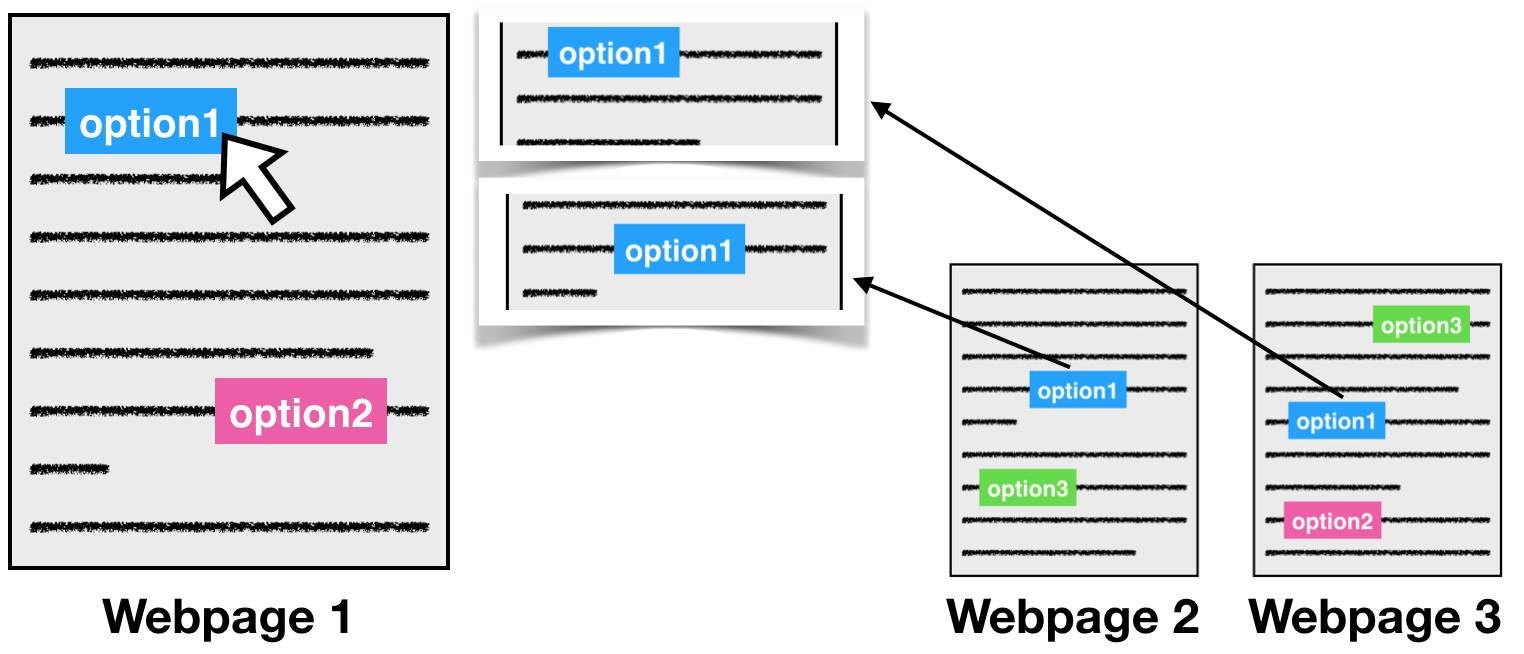
\includegraphics[width=0.6\textwidth]{images/gather.png}
    \caption{The gather mechanism gathers and presents evidence from different webpages when the user encountered a new entity.}
    \label{fig:gather}
\end{figure}



Study 1 will test a proposed mechanism called ``gather and propagate'' where the system gathers relevant evidence across webpages when the user encountered a new option (Figure \ref{fig:gather}) and propagate their notes about the option to other pages where it was also mentioned (Figure \ref{fig:propagate}).
Similar to the SearchScape system from \cref{chap:searchscape}, the gather mechanism allows users to evaluate an unfamiliar option efficiently by reviewing how it was mentioned by different sources without going through multiple webpages and look for places it was cited, but explore the benefits during reading and foraging instead of as an initial overview. The propagate mechanism allows users to re-find and re-access previously saved notes efficiently when encountering the same options again on a different webpage, lowering the cost of cross-referencing between webpages and user notes. 
A previous system that allowed users to take note in a browser sidebar across tabs has pointed to potential scaling limitations for users to re-find and re-access previously saved notes \cite{notetoself}. Participants used two strategies to re-access their notes: browsing their lists of notes and/or filtering notes with specific keywords from memory. While these strategies might be effective for small tasks with a few saved notes, they might not scale to larger tasks. The proposed study will also explore whether the entity-centric propagation mechanism will enable efficient re-access of previously created note when conducting large complex exploratory search tasks.

\begin{figure}
    \centering
    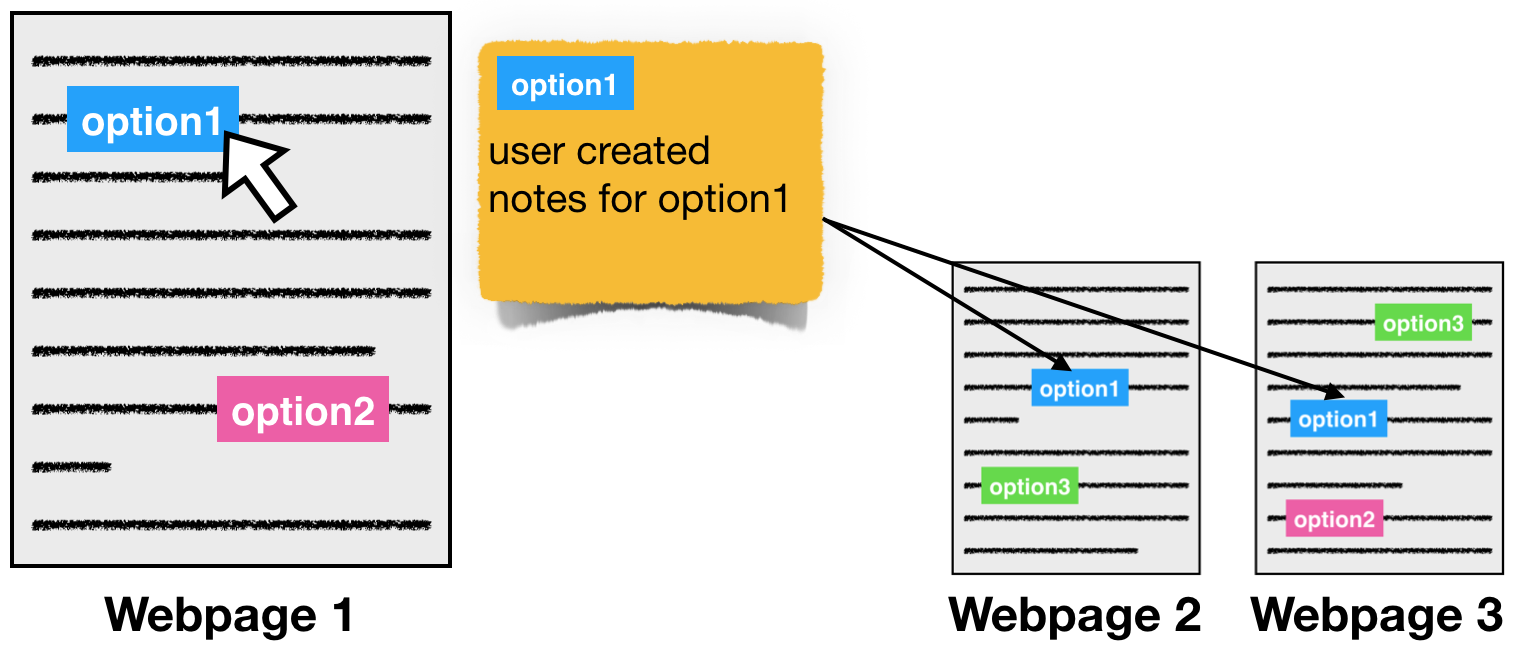
\includegraphics[width=0.6\textwidth]{images/propagate.png}
    \caption{When users take note about an option, the system propagates their notes to other webpages that also mentioned the same option for efficient re-access.}
    \label{fig:propagate}
\end{figure}
